
\documentclass[a4paper,10pt]{article}

\usepackage[utf8]{inputenc}
\usepackage{tikz}
\usepackage{latexsym}
\usepackage{amsmath}
\usepackage{amssymb}
\usepackage{amsthm}
\usepackage{tabulary}
\usepackage{algorithm}%%psedocodigo
\usepackage{algorithmic}
%\input{spanishAlgorithmic} % mi archivo de traducción
\usepackage{graphicx}



%opening
\title{Colas con priopidad (Heaps)}
\author{ \Large Luigy Alex Machaca Arcana \\Luigy.mach.arc@gmail.com \\ Universidad Nacional de San Agustín \\ Escuela Profesional de Ciencia de la Computación \\ Análisis y Estructura de Datos }

\begin{document}
\maketitle
\begin{abstract}
Los  heaps son estructuras frecuentemente usadas para implementar colas de prioridad, en dicha estructura la extracción del menor dato es mas rápida que en otras estructuras. Existen diferentes formas de implementar este tipo de estructuras, algunas de ellas son \textit{binary heap, binomial heap, fibonacci heap}. Se explicará conceptos y algunas funciones sobre estas estructuras.
\end{abstract}

\section{Introducción}

A veces necesitamos usar estructuras parcialmente ordenadas para recurrir al elemento con mayor prioridad.
Por ejemplo para el algoritmo de Kruskal y Prim para el cálculo del
árbol de expansión mínimo de un grafo etiquetado, ó para el algoritmo de Dijkstra para el cálculo de caminos
mínimos en un grafo etiquetado, por lo que las aristas deben estar almacenadas en una estructura parcialmente ordenada. Otro caso se da cuando queremos establecer orden de prioridad en un grupo de elementos, de tal forma que podemos obtener un cierto numero de elementos con la mayor prioridad. Entre este tipo de estructuras se encuentran las \textit{priority queues} \footnote{\textbf{Una cola de prioridades} que es una estructura de datos en la que los elementos se atienden en el orden indicado por una prioridad asociada a cada uno}, tales como listas enlazadas, binary heaps, binomial heaps, fibonacci heaps.\cite{diapos} Las estructuras a analizar en este artículo son: Binary Heap, la cuales estan basadas en un árbol binario; y Binomial Heap, que está basada en un arboles binomiales. Un dato extra es que es posible ordenar elementos haciendo uso de las funciones de heaps.

\section{Conceptos previos}
\subsection{Priority queue}
Priority Queue es una estructura de datos fundamental que permite el acceso solo al elemento mínimo.  \cite{cormen}
Una implementación de las priority queue es el Heap, que debe soportar inserción, consultar menor y extraer menor.


\subsection{Heaps}
Un Heap es una estructura de datos basada en árboles (\textit{se utilizan para el ordenamiento de datos \textit{HeapSort} y para implementar colas de prioridades} ), estas satisface la siguiente propiedad: Para todo nodo A cuyo padre es P, P debe tener mayor prioridad que A. 

\subsection{Binary Heap}
Un binary heaps es un caso particular y bastante sencillo, dicha estructura esta basada en un árbol  binario parcialmente ordenado, que puede verse como un árbol binario con dos propiedades(Restricciones) adicionales\cite{AEDc++} :
\begin{itemize}
	\item Cada nodo tiene un valor mayor o menor 		(orden ascendente u orden descendente) que cualquiera de sus hijos.
	\item Este árbol binario tiene que tiene que ser completo, es decir debe tener todos sus nodos, con
excepción de que tal ves no existan todos los nodos en el último nivel.	
\end{itemize}
Cumpliendo estas anteriores propiedades el Binary Heap se puede representar a través de un vector como se muestra en la Figura \ref{fig:heapMax}.
A partir de esto se puede deducir que:
\begin{itemize}
	\item Para cada elemento en la posicion i \footnote{como \textbf{i} es la poscion siempre sera un entero.}  .
	\item Sus hijo deben de estar(dentro del array), en las posiciones \textbf{2k} y \textbf{2k+1}, siendo el primero para hijo izquierdo y el segundo para el derecho respectivamente.
	\item para encontrar el padre de k solo se debe realizar una división entera del índice k/2.
\end{itemize}


\begin{figure}[!ht]
	\caption{Max Heap, representado a través de un array}
	\label{fig:heapMax}
	\begin{center}
	  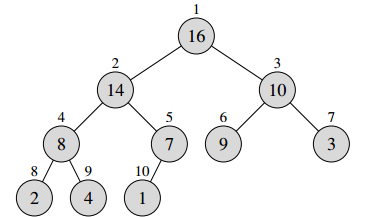
\includegraphics[scale=0.6]{heap_maximo.jpg}	
	 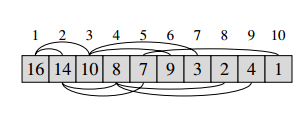
\includegraphics[width=0.6\textwidth]{heap_array.jpg}
	\end{center}	
\end{figure}


Para el binary heap una de las operaciones más importantes es \textbf{Heapify}, que
se encarga de hacer que se cumpla la propiedad de los Heaps En el Algoritmo (\ref{alg:algoritmoHeapify}) se expone el pseudocódigo.
Para extraer la cabeza del heap, simplemente se intercambia, el último elemento del heap con el primero para luego eliminar este último y aplicar Heapify(\ref{alg:algoritmoHeapify}) y todo el árbol.

\begin{algorithm}[!h]
	
	\caption{Heapity} \label{alg:algoritmoHeapify}
	\begin{algorithmic} 
\REQUIRE $data$ (Vector de datos) , $i$ (Posición del nodo a calcular) , $cmp$ (Función de Comparación)
\STATE $l \leftarrow 2*i$
\STATE $r \leftarrow 2*i+1$
\STATE $temp \leftarrow i$
\IF{$l<n$ AND $cmp(data[l],data[temp])$}
\STATE $temp \leftarrow l$
\ENDIF
\IF{$r<n$ AND $cmp(data[r],data[temp])$}
\STATE $temp \leftarrow r$
\ENDIF
\IF{$temp=i$}
\STATE $return$
\ENDIF
\STATE $swap(data[i],data[temp])$
\STATE $Heapify(data,temp,cmp)$
\end{algorithmic}
\end{algorithm}

	Otra de las operaciones importantes es la interseción, la cual añade el elemento al final del árbol para luego hacerlo flotar \footnote{ por flotar, revisar que arbol cumple las condiciones necesarias} hasta que llegue a la posición correcta.

En el Algoritmo (\ref{alg:algoritmo_flotar}) se expone el pseudocódigo.

\begin{algorithm}[!h]
	
	\caption{insert} \label{alg:algoritmo_flotar}
	\begin{algorithmic} 
\REQUIRE $data$ (Vector de datos) , $key$ (Dato a insertar) , $cmp$ (Función de Comparación)
\STATE $data.push_back(key)$
\FOR{$j=data.size()-1;j>0$ AND $cmp(data[j],data[j/2]);j=j/2$}
\STATE $swap(data[j],data[j/2])$
\ENDFOR
\end{algorithmic}
	
\end{algorithm}

\section{Binomial Heap}
Estan basados en arboles binomiales, los cuales son árboles definidos recursivamente. Si $B_k$ es un árbol binomial, $B_0$ será un solo nodo y para $k>0$, $B_k$ tendrá dos $B_{(k-1)}s$ que estarán unidos entre sí de tal manera que la raíz de uno es el hijo izquierdo de la raíz de la otra. Algunos ejemplos en la figura \ref{fig:ArbolBinomial}.

\begin{figure}[!ht]
%cambiar por la imagen de un arboll binomial%
	\caption{Arboles binomiales}
	\label{fig:ArbolBinomial}
	\begin{center}
	  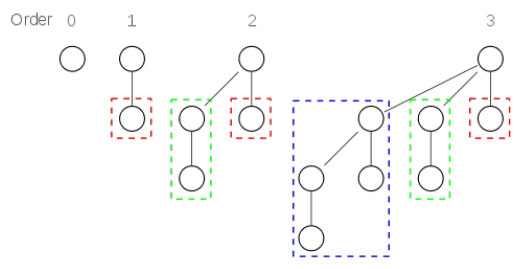
\includegraphics[scale=1.7]{arbol_binomial.jpg}	
	\end{center}	
\end{figure}

El binomial heap es un conjunto de arboles binomiales parcialmente ordenados, y contiene no ,ás de un árbol binomial para cada grado del heap. Las operaciones de este heap estan basadas en la operación de unión. La inserción es la unión de un heap con otro heap con un solo nodo. Al momento de enlazar los árboles se debe mantener las prioridades.

\section{Comparacíon}
	Ambos Heaps tienen el mismo costo computacional de todas sus funciones con un excepcion de la unión. A continuación se presenta la tabla de comparación de costos computacionales en el peor y mejor caso entre binary y binomial heap.
\vspace{5mm}
\newline
\begin{tabular}{| l | c | c| }
 \hline                        
  Función & Binary Heap (Peor caso) & Binomial Heap (Peor Caso) \\
  \hline
  Insert & $\log(n)$ & $\log(n)$ \\
  Encontrar mínimo & $1$ & $\log(n)$ \\
  Extraer mínimo & $\log(n)$ & $\log(n)$ \\
  Union & $n$ & $\log(n)$ \\
  \hline
\end{tabular} 
	
	
	
	




\newpage
\begin{thebibliography}{9}

\bibitem[1]{cormen}
Thomas H. Cormen, Charles E. Leiserson, Ronald L. Rivest, Cliford Stein.
\textit{Introduction to Algorithms}. The MIT Press, Cambridge, Massachusetts, 3rd
Edition, 2009.

\bibitem[2]{diapos}
Kevin Wayne,\textit{ Binary and Binomial Heaps - Theory of Algorithms}. Princeton
University, 2002.

\bibitem[3]{AEDc++}
Antonio Garrido Carrillo y Joaquin Valdivia , Antonio Garrido Carrillo, Joaquín Fernández Valdivia
\textit{Abstracción y Estructuras de datos en C++}
Delta Publicaciones, 2006 .

\bibitem[4]{priorityQueue}
Alonso Ramirez Manzanares \textit{Colas de prioridad ( priority queues)} - Computación y Algoritmos, 2012.


	\end{thebibliography}
	
	
	
\end{document}



